\documentclass[10.5pt,a4paper]{ctexart}
\usepackage{ctex}
\usepackage{emptypage} 
\usepackage{fancyhdr}
\usepackage{amsmath,amsfonts,amssymb}
\usepackage{graphicx}
\usepackage{mathptmx}
\usepackage{booktabs}
\usepackage[labelfont=bf]{caption}
\usepackage{indentfirst}
\usepackage{caption}
\usepackage{enumitem}
\usepackage[marginal]{footmisc}
\usepackage{subfigure}
\usepackage{fontspec}
\usepackage{geometry}
\usepackage{setspace}
\usepackage{hyperref}
\usepackage{caption}
\usepackage{subfigure}
\hypersetup{
    colorlinks=true,
    linkcolor=blue,
    filecolor=blue,      
    urlcolor=cyan,
    citecolor=cyan,
}
\newgeometry{left=3.5cm,top=2.5cm,bottom=2.5cm,right=2.5cm}
\setmainfont{Times New Roman}
%\setCJKmainfont[BoldFont=SimHei,ItalicFont=KaiTi]{SimSun}


\setlength{\textwidth}{17.00cm}
\setlength{\textheight}{24.50cm}

\renewcommand{\baselinestretch}{2}


\title{\textbf{\Huge{基于双摆系统初探楼体阻尼器工作原理}}}
\author{
	\Large{姓名:张明轩}\qquad 
	\Large{学号:211240005}\\[8pt]
	\Large{所在院(系):匡亚明学院}\\[16pt]
}

\date{}
\newcommand{\supercite}[1]{\textsuperscript{\cite{#1}}}

\begin{document}
\maketitle


\setlength{\oddsidemargin}{-.5cm} 
\setlength{\evensidemargin}{\oddsidemargin}
\setlength{\textwidth}{17.00cm}

\section{摘要}
\noindent 本文首先将楼体---阻尼器模型简化为倒立复摆+单摆的模型, 对其进行数学建模. 在此基础上, 调用scipy库对得到的微分方程进行数值求解, 利用仿真数据验证模型的正确性. 
接着本文将在模型中加入周期变化的驱动力, 以模拟地震波, 并对该模型进行小角度近似,给出在小角度情况下的运动方程, 并简述基于此运动方程分析楼体稳定性与各参数间关系的思路.\\
\noindent \textbf{关键词:} 双摆模型,阻尼器,仿真测试
\section{引言}

\noindent \textbf{研究的问题的主要背景情况和意义:}
双摆模型, 是由一个单摆连接在另一个单摆末端所构成的系统, 是一种具有混沌系统的简单动力系统. 其系统构成相对简单, 但运动过程却极其复杂,无法用公式准确预测物体的行径, 
初始条件的细微区别都会导致系统运动的巨大差异\cite{ref1}. 双摆系统在生活中有许多实例, 例如摆车上的挂钩与货物构成的双摆系统, 大楼阻尼器与楼体构成的双摆系统等. 利用双摆模型进行分析, 
能够提高实际应用中的准确性\cite{ref2}. 本文将主要着眼阻尼器---楼体双摆系统, 在现有各类阻尼器研究\cite{ref3} \cite{ref4}的基础上, 简化模型, 分析其防风抗震的基本原理, 并分析如何通过控制摆锤质量和悬线长度, 来使得楼体在面对多变的震动情况时, 能够更好的应对.\\
\noindent \textbf{主要的研究目标:}
初步建立阻尼器---楼体双摆系统的数学模型, 并通过仿真验证其正确性; 在小角度情况下对模型线性化, 得出双摆系统的近似运动方程,并分析如何在该运动方程的基础上, 确定摆锤质量, 悬线长度, 以保证地震波对大楼的影响最小.
\section{正文}

\subsection*{1.双摆模型的建立与模拟}
在详细研究有关设计之前, 需要对该问题的核心---双摆系统进行研究分析. 本节将首先对大楼---摆锤双摆系统进行数学建模; 
然后通过数值积分的方法, 调用\href{https://docs.scipy.org/doc/scipy/tutorial/integrate.html}{scipy.integrate库}\cite{ref5}, 对该模型进行简单模拟, 以验证模型的正确性.
\subsubsection*{数学建模}
\begin{figure}[htbp]
	\begin{center}
		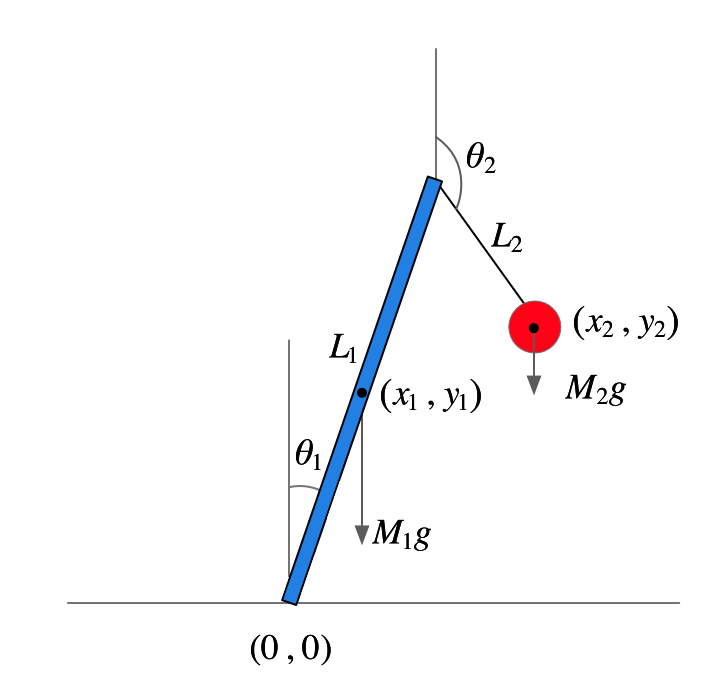
\includegraphics[width=3in]{figs/primary.png}
	\end{center}
	\caption{双摆模型}
\end{figure}

如图1所示,建立双摆系统模型如下: 大楼为复摆, 质量为$M_1$, 高度为$L_1$, 与竖直方向所成夹角为$\theta_1$; 
摆锤为单摆, 质量为$M_2$, 长度为$L_2$, 与竖直方向所成夹角为$\theta_2$.由此可以表示出大楼质心和摆锤位置:\\
\begin{equation}
\left \{ 
  \begin{aligned}
  &x_1 = \frac{L_1}{2} \sin{\theta_1}\\
  &y_1 = \frac{L_1}{2} \cos{\theta_1}
  \end{aligned}
\right.
\end{equation}

\begin{equation}
\left \{ 
  \begin{aligned}
  &x_2 = L_1\sin{\theta_1} + L_2\sin{\theta_2}\\
  &y_2 = L_1\cos{\theta_1} + L_2\cos{\theta_2}
  \end{aligned}
\right.
\end{equation}
注意到, 对于整个系统, 其运动状态可以用广义坐标$\theta_1, \theta_2$及其广义速度进行描述. 
所以可以对大楼-摆锤双摆系统建立拉格朗日量: 
\begin{equation}
  \mathcal{L} = T - V
\end{equation}
其中$T$为系统的动能, $V$为系统的势能.将(1)式和(2)式带入, 可得:
\begin{equation}
\begin{split}
  \mathcal{L} = \frac{1}{2} M_1 v_1^2 + \frac{1}{2} M_2 v_2^2 + \frac{1}{2} I_1 \dot{\theta_1}^2 - M_1 g y_1 - M_2 g y_2\\
\end{split}
\end{equation}
大楼的模型简化为均匀杆, 其转动惯量$I_1$为$\displaystyle\frac{1}{12} M_1 L_1^2$, 而$v_1, v_2$可以由物体的位置坐标求导得到:
\begin{equation}
\left \{ 
  \begin{aligned}
  &v_{x_1} = \frac{L_1}{2}\dot{\theta_1}\cos{\theta_1}\\
  &v_{y_1} = -\frac{L_1}{2}\dot{\theta_1}\sin{\theta_1}
  \end{aligned}
\right.
\end{equation}

\begin{equation}
\left \{ 
  \begin{aligned}
  &v_{x_2} = L_1\dot{\theta_1}\cos{\theta_1} + L_2\dot{\theta_2}\cos{\theta_2}\\
  &v_{y_2} = -L_1\dot{\theta_1}\sin{\theta_1} - L_2\dot{\theta_2}\sin{\theta_2}
  \end{aligned}
\right.
\end{equation}
将上述关系带入(4)式, 可得:
\begin{equation}
\begin{split}
\mathcal{L} = \left(\frac{1}{6}M_1 + \frac{1}{2}M_2\right)L_1^2\dot{\theta_1}^2 + \frac{1}{2}M_2 L_2^2 \dot{\theta_2}^2 + M_2L_1L_2 \dot{\theta_1} \dot{\theta_2}\cos{\left(\theta_1 - \theta_2\right)} - \left(\frac{1}{2}M_1 + M_2\right)L_1 g \cos{\theta_1} - M_2 L_2 g \cos{\theta_2}
\end{split}
\end{equation}
对于广义坐标$\theta_1, \theta_2$的拉格朗日方程如下:
\begin{equation}
\left \{ 
  \begin{aligned}
  &\frac{\mathrm{d}}{\mathrm{d}t} \frac{\partial{\mathcal{L}}}{\partial{\dot{\theta_1}}} - \frac{\partial{\mathcal{L}}}{\partial{\theta_1}} = 0\\
  &\frac{\mathrm{d}}{\mathrm{d}t} \frac{\partial{\mathcal{L}}}{\partial{\dot{\theta_2}}} - \frac{\partial{\mathcal{L}}}{\partial{\theta_2}} = 0
  \end{aligned}
\right.
\end{equation}
\begin{equation}
\left \{ 
  \begin{aligned}
  &\left(\frac{1}{3}M_1 + M_2\right) L_1^2 \ddot{\theta_1} + M_2 L_1 L_2 \dot{\theta_2}^2 \sin\left(\theta_1 - \theta_2\right) + M_2 L_1 L_2 \ddot{\theta_2}\cos{\left(\theta_1 - \theta_2\right)} - (\frac{1}{2}M_1 + M_2) L_1 g \sin{\theta_1} = 0\\
  &M_2 L_2^2 \ddot{\theta_2}^2 - M_2 L_1 L_2 \dot{\theta_1}^2 \sin{\left(\theta_1 - \theta_2\right)} + M_2 L_1 L_2 \ddot{\theta_1}\cos{\left(\theta_1 - \theta_2\right)} - M_2 L_2 g \sin{\theta_2} = 0
  \end{aligned}
\right.
\end{equation}

\subsubsection*{模拟验证}
因为双摆系统的运动属于混沌运动, 所以无法得到用以表示物体位置的$\theta_1, \theta_2$对于时间$t$的显式解. 故此处直接对(9)式中的微分方程求数值解.
而scipy.integrate库无法处理二阶微分方程, 所以此处对(9)式进行变形处理, 转化成4个一阶微分方程.
\begin{equation}
\left \{ 
  \begin{aligned}
  &\dot{\theta_1} = \omega_1\\
  &\dot{\theta_2} = \omega_2\\
  &\left(\frac{1}{3}M_1 + M_2\right) L_1^2 \dot{\omega_1} + M_2 L_1 L_2 \omega_2^2 \sin\left(\theta_1 - \theta_2\right) + M_2 L_1 L_2 \dot{\omega_2}\cos{\left(\theta_1 - \theta_2\right)} - (\frac{1}{2}M_1 + M_2) L_1 g\sin{\theta_1} = 0\\
  &M_2 L_2^2 \dot{\omega_2}^2 - M_2 L_1 L_2 \omega_1^2 \sin{\left(\theta_1 - \theta_2\right)} + M_2 L_1 L_2 \dot{\omega_1}\cos{\left(\theta_1 - \theta_2\right)} - M_2 L_2 g \sin{\theta_2} = 0
  \end{aligned}
\right.
\end{equation}
每一组模拟中, 保证$\theta_1, \theta_2$初始情况下一致.总共完成两组模拟(\href{https://github.com/zhangmxxx/Physics-paper-2022}{source code}):\\
1. $\theta_1 = 0.01, \theta_2 = \pi$, $L_1 : L_2$保持为$100:1$, 设置$M_1:M_2$为$1:1, 2:1, 10:1, 100:1$\\
2. $\theta_1 = 0.1, \theta_2 = \pi$, $M_1 : M_2$保持为$10:1$, 设置$L_1:L_2$为$100:1, 100:2, 100:10, 100:50$\\
得出仿真结果如下:\\
\begin{figure}[htbp] \centering    
  \subfigure[$M_1:M_2 = 1:1$] {
   \label{fig:1-1}     
  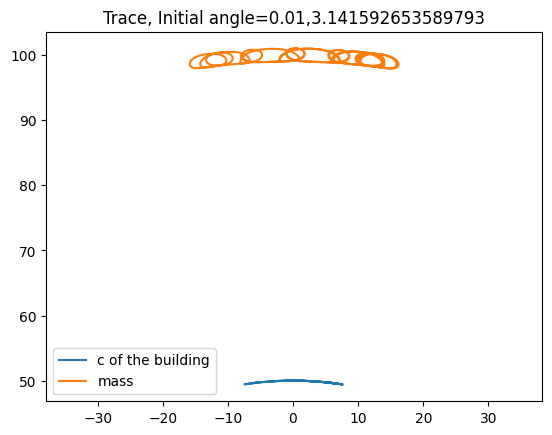
\includegraphics[width=0.4\columnwidth]{figs/1-1.png}  
  }     
  \subfigure[$M_1:M_2 = 2:1$] { 
  \label{fig:1-2}     
  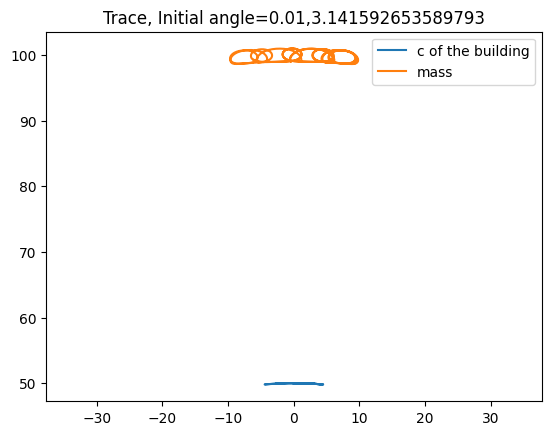
\includegraphics[width=0.4\columnwidth]{figs/1-2.png}     
  }    \\
  \subfigure[$M_1:M_2 = 10:1$] { 
  \label{fig:1-3}     
  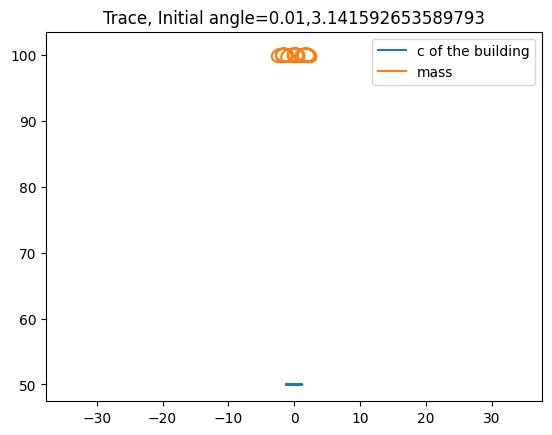
\includegraphics[width=0.4\columnwidth]{figs/1-3.png}     
  }   
  \subfigure[$M_1:M_2 = 100:1$] { 
  \label{fig:1-4}     
  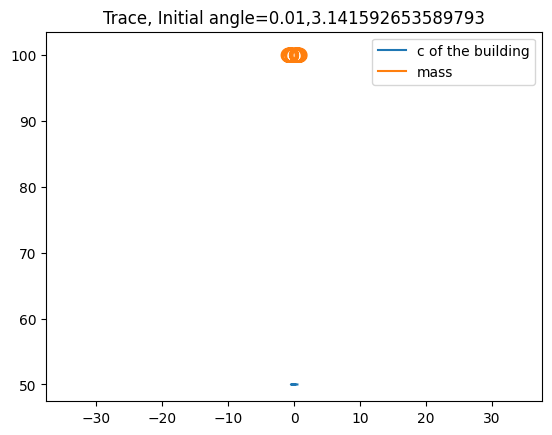
\includegraphics[width=0.4\columnwidth]{figs/1-4.png}     
  }   
  \caption{$L_1 : L_2 = 100 : 1$}     
  \label{fig:1}     
\end{figure}

\newpage

\begin{figure}[htbp] \centering    
  \subfigure[$L_1:L_2 = 100:1$] {
   \label{fig:2-1}     
  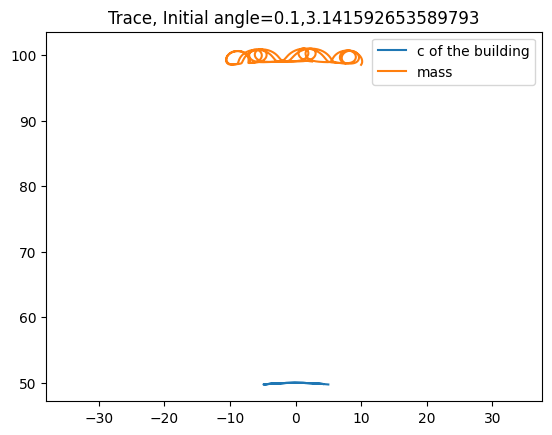
\includegraphics[width=0.4\columnwidth]{figs/2-1.png}  
  }     
  \subfigure[$L_1:L_2 = 100:2$] { 
  \label{fig:2-2}     
  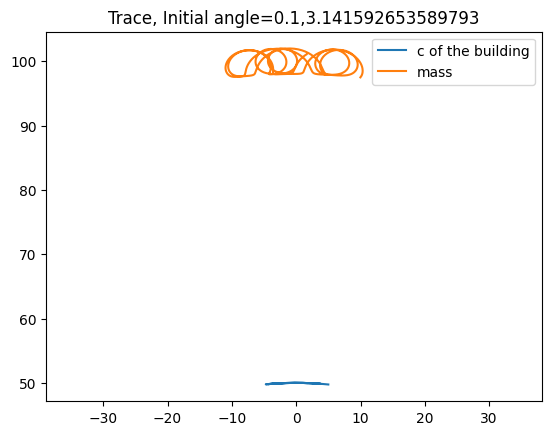
\includegraphics[width=0.4\columnwidth]{figs/2-2.png}     
  }    \\
  \subfigure[$L_1:L_2 = 100:10$] { 
  \label{fig:2-3}     
  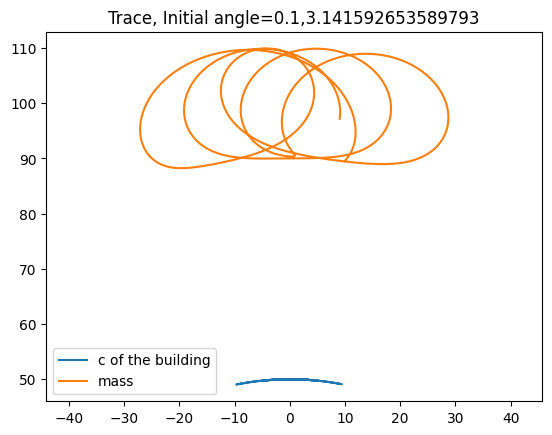
\includegraphics[width=0.4\columnwidth]{figs/2-3.png}     
  }   
  \subfigure[$L_1:L_2 = 100:50$] { 
  \label{fig:2-4}     
  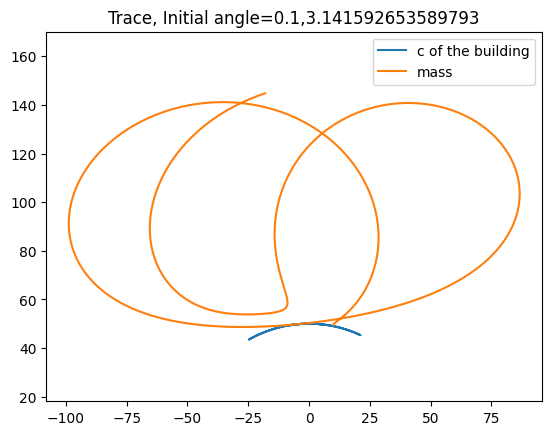
\includegraphics[width=0.4\columnwidth]{figs/2-4.png}     
  }   
  \caption{$M_1 : M_2 = 10 : 1$}     
  \label{fig:2}     
\end{figure}
\subsubsection*{模拟验证总结}
以楼体质心运动轨迹的$x$坐标的最值大小作为楼体摇晃幅度的衡量指标.从第一组模拟结果可知:\\
$M_1:M_2$从$1:1$至$10:1$时, 随着大楼质量的增加, 楼体摇晃幅度显著减小, 
$M_1:M_2$从$10:1$至$100:1$时, 随着大楼质量的增加, 楼体摇晃幅度仍有减小, 但减小幅度不显著; 从第二组模拟结果可知: $L_1:L_2$从$100:50$至$100:1$时, 
随着楼体与悬线长度之比的增加, 楼体摇晃幅度显著减小, 同时也可以看到, 阻尼器摆动的周期显著减小. 综上所述,模拟结果基本符合实际, 模型建立基本正确.
\newpage
\subsection*{2.进一步探究}
上一部分的模型分析了在无驱动力作用的情况下, 双摆系统的数学模型和运动情况. 但在实际中, 面对例如强风, 地震的自然灾害, 大楼还会受到外界驱动力的作用.
本节将首先在上一部分的模型中加入周期性驱动力$F = F_0\sin{\left(\omega t + \varphi \right)}$以优化模型; 接着, 将在小角度近似的情况下, 对模型进行线性化处理,  
得出该系统的运动情况. 最后, 将尝试给出分析悬线长L, 阻尼器质量M对大楼稳定性影响的简要思路.
\subsubsection*{模型优化}
\begin{figure}[htbp]
	\begin{center}
		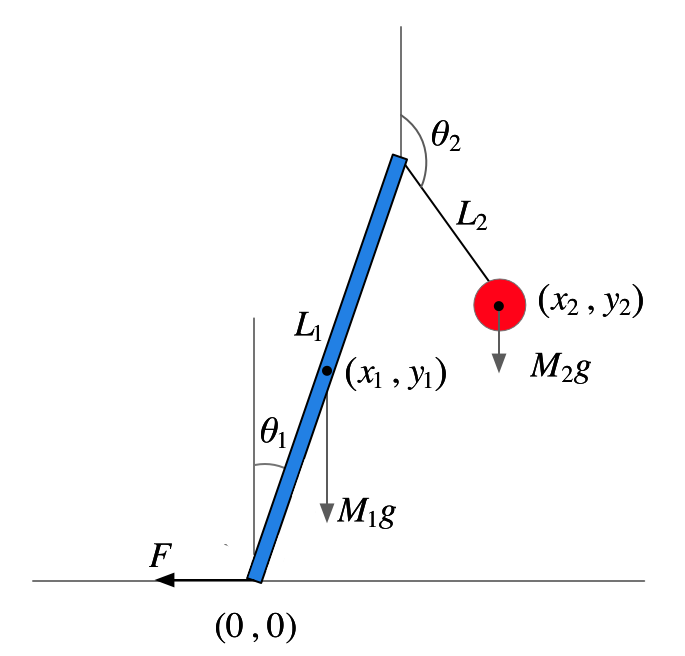
\includegraphics[width=3in]{figs/plusforce.png}
	\end{center}
	\caption{加入驱动力的双摆模型}
\end{figure}
驱动力$F = F_0\sin{\left(\omega t + \varphi \right)}$为非保守力, 所以只需要将(8)式中第一个方程修改为:\\
\begin{equation}
  \begin{aligned}
  &\frac{\mathrm{d}}{\mathrm{d}t} \frac{\partial{\mathcal{L}}}{\partial{\dot{\theta_1}}} - \frac{\partial{\mathcal{L}}}{\partial{\theta_1}} = F_0\sin{\left(\omega t\right)}\\
  \end{aligned}
\end{equation}
注意到(11)式右边存在变量$t$, 而$t$无法通过$t(\theta_1, \theta_2, \dot{\theta_1}, \dot{\theta_2})$显式表示, 所以无法沿用上一节的处理方式, 从而对
得到的微分方程进行数值求解, 模拟系统运动过程.考虑到现实中, 地震,强风等自然因素对楼体造成的扰动较小,即$\theta_1, \theta_2 - \pi$均为小量.取$\theta_3 = \theta_2 - \pi$, 则$\theta_3$也为小量.
故存在以下近似式: $\displaystyle \cos{\left(\theta_1 - \theta_2\right)} = \cos{\left(\theta_1 - \pi - \theta_3\right)} = -\cos{\left(\theta_1 - \theta_3\right)} \approx -1$, 
$\displaystyle\cos{\theta_1} \approx 1 - \frac{1}{2}\theta_1^2$, $\displaystyle\cos{\theta_2} \approx \frac{1}{2}\theta_3^2 - 1$.根据以上近似式, 可以将(7)式在$\theta_1 = 0$, $\theta_2 = \pi$处进行泰勒展开, 并保留线性项和二次项:
\begin{equation}
\begin{split}
\mathcal{L} & = \left(\frac{1}{6}M_1 + \frac{1}{2}M_2\right)L_1^2\dot{\theta_1}^2 + \frac{1}{2}M_2 L_2^2 \dot{\theta_2}^2 + M_2L_1L_2 \dot{\theta_1} \dot{\theta_2}\cos{\left(\theta_1 - \theta_2\right)} - \left(\frac{1}{2}M_1 + M_2\right)L_1 g \cos{\theta_1} - M_2 L_2 g \cos{\theta_2} \\
& = \left(\frac{1}{6}M_1 + \frac{1}{2}M_2\right)L_1^2\dot{\theta_1}^2 + \frac{1}{2}M_2 L_2^2 \dot{\theta_3}^2 - M_2L_1L_2 \dot{\theta_1} \dot{\theta_3} - \left(\frac{1}{2}M_1 + M_2\right)L_1 g \left(1 - \frac{1}{2} \theta_1^2\right) + M_2 L_2 g \left(1 - \frac{1}{2}\theta_3^2 \right) \\
& = \left(\frac{1}{6}M_1 + \frac{1}{2}M_2\right)L_1^2\dot{\theta_1}^2 + \frac{1}{2}M_2 L_2^2 \dot{\theta_3}^2 - M_2L_1L_2 \dot{\theta_1} \dot{\theta_3} + \left(\frac{1}{4}M_1 + \frac{1}{2}M_2\right) L_1 g \theta_1^2 - \frac{1}{2}M_2 L_2 g \theta_3^2 \\ 
& - \left(\frac{1}{2}M_1 + M_2\right) L_1 g  + M_2 L_2 g
\end{split}
\end{equation}
对该表达式列出相应的拉格朗日方程, 可得:
\begin{equation}
\left \{ 
  \begin{aligned}
  &\left(\frac{1}{3}M_1 + M_2\right) L_1^2 \ddot{\theta_1}  - M_2 L_1 L_2 \ddot{\theta_3} - (\frac{1}{2}M_1 + M_2) L_1 g \theta_1 = F_0 \sin{\left(\omega t\right)}\\
  &-M_2L_1L_2\ddot{\theta_1} + M_2L_2^2\ddot{\theta_3}  + M_2L_2g\theta_3 = 0
  \end{aligned}
\right.
\end{equation}
令 $\theta(t) = \begin{bmatrix} \theta_1(t) \\ \theta_3(t) \end{bmatrix}$, $\displaystyle M = \begin{bmatrix} \left(\frac{1}{3}M_1 + M_2 L_1^2 \right) & -M_2L_1L_2\\-M_2L_1L_2 &  M_2L_2^2\end{bmatrix}$,
$K = \begin{bmatrix} -\left(\frac{1}{2}M_1 + M_2\right)L_1g & 0 \\ 0 & M_2L_2g\end{bmatrix}$ , $F = \begin{bmatrix} F_0\sin{\left(\omega t\right)} \\ 0\end{bmatrix}$, \\\\则(13)式可以表示为:
\begin{equation}
  \begin{aligned}
  & M \ddot{\theta} + K \theta = F
  \end{aligned}
\end{equation}
该表达式形式与振子受迫振动表达式形式一致.猜想$\theta_1, \theta_3$在0附近的随时间做正弦变化.故取$\theta_1, \theta_3$的试探解为$\theta_1 = A_1\sin{\left(\omega t + \varphi_1\right)}$, $\theta_3 = A_3\sin{\left(\omega t + \varphi_3\right)}$\cite{ref6}, 代入(13)式并整理可得:
\begin{equation}
\left \{ 
  \begin{aligned}
  &\left[-\left(\frac{1}{3}M_1 + M_2\right)L_1^2A_1\omega^2 \cos{\varphi_1} + M_2L_1L_2A_3\omega^2\cos{\varphi_3} - \left(\frac{1}{2}M_1 + M_2\right)L_1A_1g\cos{\varphi_1} - F_0\right]\sin{\left(\omega t\right)}\\
  &+ \left[-\left(\frac{1}{3}M_1 + M_2\right)L_1^2A_1\omega^2 \sin{\varphi_1} + M_2L_1L_2A_3\omega^2\sin{\varphi_3} - \left(\frac{1}{2}M_1 + M_2\right)L_1A_1g\sin{\varphi_1} \right]\cos{\left(\omega t\right)} = 0\\
  &\left(M_2L_1L_2A_1\omega^2\cos{\varphi_1} - M_2L_2^2A_3\omega^2\cos{\varphi_3} + M_2L_2gA_3\cos{\varphi_3}\right)\sin{\left(\omega t\right)}\\
  &+ \left(M_2L_1L_2A_1\omega^2\sin{\varphi_1} - M_2L_2^2A_3\omega^2\sin{\varphi_3} + M_2L_2gA_3\sin{\varphi_3}\right)\cos{\left(\omega t\right)} = 0
  \end{aligned}
\right.
\end{equation}
因为$\sin{\left(\omega t\right)}$, $\cos{\left(\omega t\right)}$项的系数均为与时间无关的常数, 所以系数均为0, 由此可得:
\begin{equation}
\left \{ 
  \begin{aligned}
  & \left[-\left(\frac{1}{3}M_1 + M_2\right)L_1^2A_1\omega^2 \cos{\varphi_1} + M_2L_1L_2A_3\omega^2\cos{\varphi_3} - \left(\frac{1}{2}M_1 + M_2\right)L_1A_1g\cos{\varphi_1} - F_0\right] = 0 \\
  & \left[-\left(\frac{1}{3}M_1 + M_2\right)L_1^2A_1\omega^2 \sin{\varphi_1} + M_2L_1L_2A_3\omega^2\sin{\varphi_3} - \left(\frac{1}{2}M_1 + M_2\right)L_1A_1g\sin{\varphi_1} \right] = 0\\
  & \left(M_2L_1L_2A_1\omega^2\cos{\varphi_1} - M_2L_2^2A_3\omega^2\cos{\varphi_3} + M_2L_2gA_3\cos{\varphi_3}\right) = 0\\
  & \left(M_2L_1L_2A_1\omega^2\sin{\varphi_1} - M_2L_2^2A_3\omega^2\sin{\varphi_3} + M_2L_2gA_3\sin{\varphi_3}\right) = 0
  \end{aligned}
\right.
\end{equation}
解得:
\begin{equation}
\left \{ 
  \begin{aligned}
    &\varphi_1 = 0 \\
    &\varphi_3 = -\pi \\
    &A_1 = - \frac{F_0}{\left(\frac{1}{3}M_1 + M_2\right)\omega^2L_1^2 + \frac{M_2L_1^2L_2\omega^4}{g - \omega^2L_2} + \left(\frac{1}{2}M_1 + M_2\right)L_1g}\\
    &A_3 = \frac{\omega^2L_1}{g - \omega^2L_2} A_1
  \end{aligned}
\right.
\end{equation}
而在原模型中, 设$\theta_2 = A_2\sin{\left(\omega t + \varphi_2\right)}$, 则有$A_2 = A_3, \varphi_2 = \pi + \varphi_3 = 0$
\subsubsection*{稳定性分析的思路简述}
以楼体质心运动轨迹的$x$坐标的最值大小作为楼体稳定性的衡量指标. 因为$\displaystyle x_c = \frac{1}{2}L_1\sin{\theta_1}$, 所以$|x_{max}| \propto |\theta_{1_{max}}| \propto |A_1|$.
模型中的参数包括阻尼器与楼体的质量比$\displaystyle\alpha = \frac{M_2}{M_1}$, 悬线长度与楼体高度的比值$\displaystyle\beta = \frac{L_2}{L_1}$, 地震波施加的驱动力的大小$F_0$, 频率$\omega$.
若要分析稳定性与这些参数之间的关系, 只需要将$\alpha, \beta, F_0, \omega$等参数作为变量, 分析$|A_1|$的变化情况即可.

\section{总结}
通过模拟检验, 将楼体---阻尼器系统简化为倒立复摆+单摆的模型的做法基本正确. 而在存在周期性驱动力的情况下, 暂未找到合适的方法对该非线性问题进行精确求解或通过计算机进行数值求解.
但通过对双摆系统在$\theta_1 = 0$, $\theta_2 = \pi$处进行线性化,可以得出$\theta_1, \theta_2$与$t$之间的显式函数关系. 基于此关系, 可以进一步分析楼体稳定性与阻尼器质量, 悬线长度等参数的关系.

\noindent \begin{thebibliography}{99}
  \bibitem{ref1} {https://en.wikipedia.org/wiki/Double\_pendulum}
  \bibitem{ref2} {Thomas, M., \& Sawodny, O. (2022). Flatness-based feedforward and modal model-predictive state-feedback control of a double pendulum bridge crane. IFAC-PapersOnLine, 55(27), 19–24. https://doi.org/10.1016/j.ifacol.2022.10.482}
  \bibitem{ref3} {Koutsoloukas, L., Nikitas, N., \& Aristidou, P. (2022). Passive, semi-active, active and hybrid mass dampers: A literature review with associated applications on building-like structures. Developments in the Built Environment, 12, 100094. https://doi.org/10.1016/j.dibe.2022.100094}
  \bibitem{ref4} {Bitaraf, M., \& Hurlebaus, S. (2013). Semi-active adaptive control of seismically excited 20-story nonlinear building. Engineering Structures, 56, 2107–2118. https://doi.org/10.1016/j.engstruct.2013.08.031}
  \bibitem{ref5} {https://docs.scipy.org/doc/scipy/tutorial/integrate.html}
  \bibitem{ref6} {大学物理学 /卢德馨. ---2版. ---北京: 高等教育出版社, 2003.7}
	\bibitem{ref7} {https://math24.net/double-pendulum.html}
  \bibitem{ref8} {Sonmez, E., Nagarajaiah, S., Sun, C., \& Basu, B. (2016). A study on semi-active Tuned Liquid Column Dampers (sTLCDs) for structural response reduction under random excitations. Journal of Sound and Vibration, 362, 1–15. https://doi.org/10.1016/j.jsv.2015.09.020}
\end{thebibliography}
\end{document}
